
\documentclass[a4paper,12pt,firamath,article]{nsi}
\begin{document}
\titre{Le jeu de Marienbad}
\classe{NSI2}
\maketitle
\begin{center}
    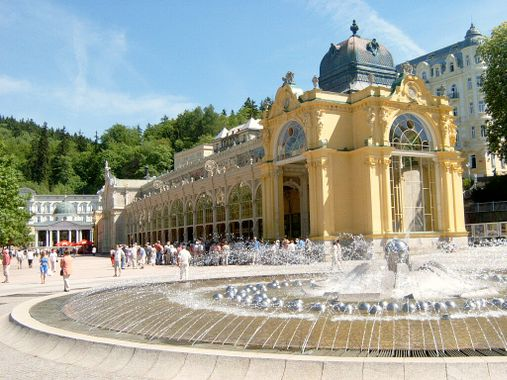
\includegraphics[width = 10cm]{img/marienbad}\\
    \footnotesize Marienbad, station thermale située en République Tchèque.
\end{center}

Ce jeu – appelé également « jeu des allumettes » – nécessite deux joueurs et 21
allumettes. Les 21 allumettes sont réparties en 6 tas, avec i allumettes dans le i\eme tas : une allumette
dans le premier tas, deux dans le deuxième, etc.\\
Chacun à son tour, les joueurs piochent dans un seul tas le nombre d’allumettes
souhaité. Le joueur qui prend la dernière allumette perd la partie.\\

Votre programme devra faire jouer deux joueurs humains. Au cours du jeu, l’affichage se
présentera simplement sous la forme suivante (si Bob est l’un des deux joueurs) :\\

\texttt{tas : \ \ \ \ \ \ \ (1, 2, 3, 4, 5, 6)\\
allumettes : [0, 2, 3, 2, 4, 4]\\
-------- Prochain joueur : Bob --------\\}


\subsection*{Fichier Marienbad.py}
Ce module contient la classe Marienbad qui comprend :
\begin{itemize}
	\item 	les attributs de la classe :
			\begin{itemize}
				\item 	\texttt{tas}, de type \mintinline{python}{tuple} d’\mintinline{python}{int};
				\item \texttt{allumettes}, de type \mintinline{python}{list} d’\mintinline{python}{int};
				\item \texttt{joueurs}, de type \mintinline{python}{tuple} de \mintinline{python}{str};
				\item \texttt{tour}, un \mintinline{python}{int} qui permet d’alterner les joueurs à chaque tour (indication : il peut servir d’indice à l’attribut joueurs).
			\end{itemize}
	\item 	les méthodes de la classe :
		\begin{itemize}
			\item 	un constructeur avec des valeurs par défaut adaptées (noms des joueurs : \mintinline{python}{'joueur1'} et "\mintinline{python}{'joueur2'});
			\item 	\mintinline{python}{__str__}, qui affiche l’état du jeu en cours;
			\item 	\mintinline{python}{verifie}, qui renvoie un booléen : \mintinline{python}{True} s’il est possible d’enlever n allumettes dans le tas t, \mintinline{python}{False} sinon;
			\item 	\mintinline{python}{enlever}, qui met à jour les tas en enlevant n allumettes dans le tas t;
			\item 	\mintinline{python}{termine}, qui renvoie un booléen : \mintinline{python}{True} si le jeu est terminé, \mintinline{python}{False} sinon.
		\end{itemize}
\end{itemize}

\subsection*{Fichier jeu.py}

Dans le programme principal :
\begin{itemize}
	\item 	saisissez le nom des deux joueurs;

\item lancez le jeu (c’est une boucle tant que le jeu n’est pas terminé);\\
 	À chaque tour vous devez :
\begin{itemize}
	\item 	afficher l'état du jeu;
	\item 	demander au joueur en cours le numéro du tas t et le nombre d’allumettes
	n qu’il désire ôter;
	\item vérifier si son choix est valide, sinon expliquer l’erreur et reposer la
	question;
	\item supprimer n allumettes du tas t;
	\item vérifier si le jeu est terminé;
	 \item annoncer le gagnant (ou le perdant).
\end{itemize}
\end{itemize}
\subsection*{Faire mieux}
La classe Marienbad est assez maladroite : on doit pouvoir simplifier cette classe. Proposer, selon vos idées, des simplifications ou des améliorations.
\end{document}